\chapter{Electromagnetism}

\begin{definition}
    A \vocab{magnetic field} is a region of space within which a current-carrying conductor, a moving charge, or a permanent magnet may experience a magnetic force.
\end{definition}

A magnetic field can be represented with directed flux lines. Magnetic flux lines are always closed loops that do not start or stop in mid-space. The lines indicate the paths that a magnetic north pole would take if it is placed in the field.

\begin{definition}
    The \vocab{magnetic flux density} or \vocab{magnetic field strength} ($B$) at a point is the magnetic force per unit length of conductor per unit current carried placed perpendicular to the field at that point.
\end{definition}

Mathematically, \[B = \frac{F}{IL \sin \t},\] where $\t$ is the angle between $B$ and $I$.

The SI unit of magnetic flux density is the tesla (T), or newton per metre per ampere (N m$^{-1}$ A$^{-1}$).

\section{Magnetic Field due to Currents}

In this section, $\m_0$ is the \vocab{permeability of free space}.

\subsection{Long Straight Wire}

\begin{figure}[H]
    \centering
    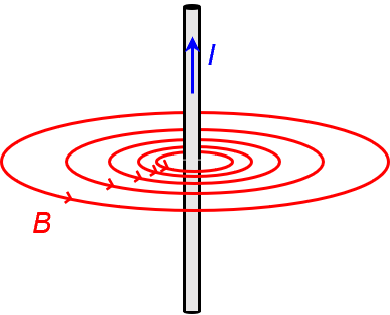
\includegraphics{media/Magnetic Field Lines - Straight Wire.png}
    \caption{The magnetic field lines for a long straight wire.\protect\footnotemark}
\end{figure}
\footnotetext{Source: \url{https://xmphysics.com/2023/01/10/14-1-1-wires-coils-and-solenoids/}}

\begin{proposition}
    The flux density $B$ at a distance $d$ from a wire is given by \[B = \m_0 \frac{I}{2\pi d}.\]
\end{proposition}

The direction of the flux around a wire can be identified using the right-hand grip rule: when the thumb of the right-hand points in the direction of the conventional current, the curled fingers point in the direction of the magnetic field lines.

\subsection{Flat Circular Coil}

\begin{figure}[H]
    \centering
    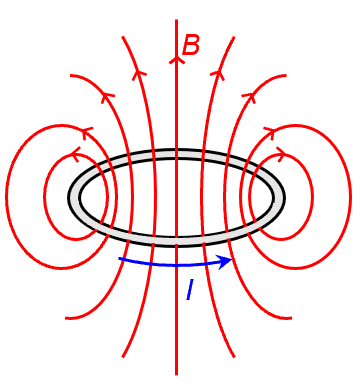
\includegraphics{media/Magnetic Field Lines - Flat Coil.png}
    \caption{The magnetic field lines for a flat circular coil.\protect\footnotemark[1]}
\end{figure}

\begin{proposition}
    The flux density $B$ at the centre of a coil with $N$ turns of radius $r$ is given by \[B = \m_0 \frac{NI}{2r}.\]
\end{proposition}

The direction of the flux can be identified using the right-hand grip rule: if the right-hand is gripping the coil so that the fingers curl in the same direction as conventional current, the extended thumb will point in the direction of the field lines inside the coil, i.e. it points to the North pole.

\subsection{Long Solenoid}

\begin{figure}[H]
    \centering
    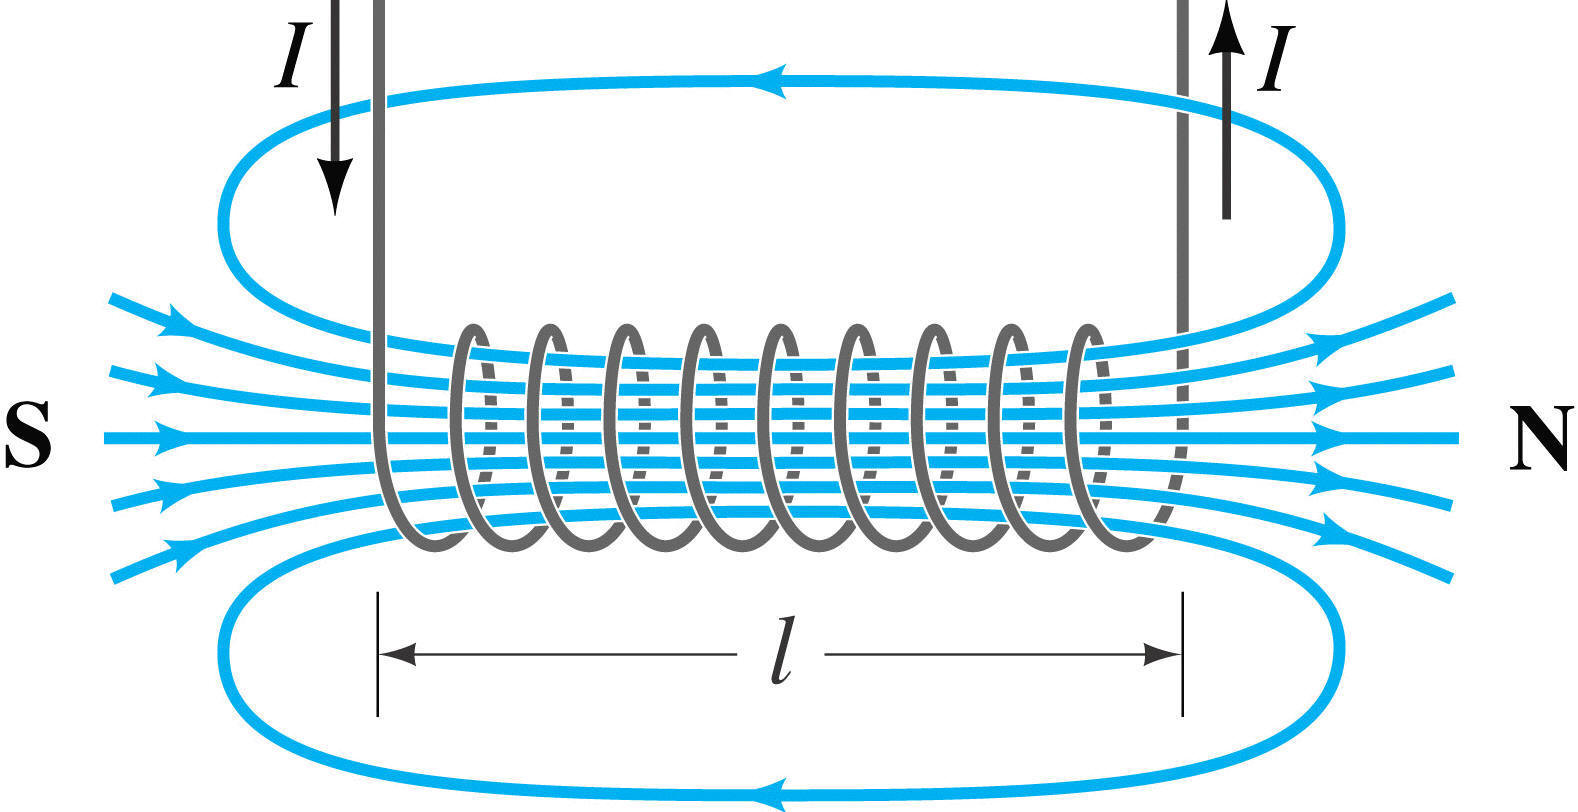
\includegraphics[scale=0.3]{media/Magnetic Field Lines - Solenoid.jpg}
    \caption{The magnetic field lines for a long solenoid.\protect\footnotemark}
\end{figure}
\footnotetext{Source: \url{https://www.miniphysics.com/ss-magnetic-field-due-to-current-in-a-solenoid.html}}

\begin{proposition}
    The flux density $B$ at the centre of a long solenoid of length $L$ with $N$ turns is given by \[B = \m_0 \frac{NI}{L}.\]
\end{proposition}

The direction of the flux can be identified using the right-hand grip rule.

The flux density inside a solenoid may be influenced by the presence of a core with a different permeability from that of free space. For instance, with a ferrous (``soft'' iron) core, which has a permeability of about $5000\m_0$, the flux density could be increased by a factor of about 5000.

Solenoids with a core of high permeability are called \vocab{electromagnets}.

\section{The Motor Effect}

\subsection{Current-Carrying Conductor}

\begin{proposition}
    A conductor of length $L$ carrying a current $I$ at an angle $\t$ to a uniform magnetic field of flux density $B$ will experience a force $F$ given by \[F = BIL\sin\t.\]
\end{proposition}
\begin{proof}
    Recall the definition of magnetic flux: \[B = \frac{F}{IL\sin\t} \implies F = BIL\sin\t.\]
\end{proof}

The direction of the magnetic force, which is perpendicular to both the field and the current, can be predicted using \vocab{Fleming's left-hand rule}: if the thumb and the first two fingers of the left hand are held so that they are mutually at right angles, then they represent force ($F$), field ($B$) and current ($I$) respectively.

\subsubsection{Current Balance}

The force on a current-carrying conductor can be used to measure the flux density of a magnetic field using a \vocab{current balance}.

\begin{figure}[H]
    \centering
    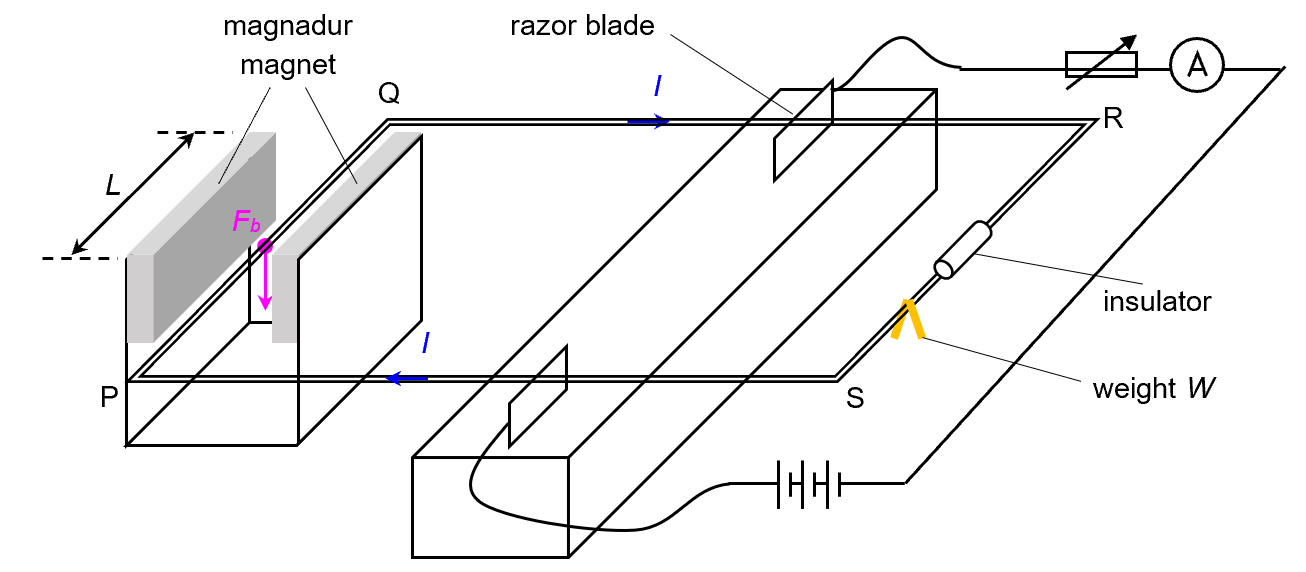
\includegraphics[scale=0.7]{media/Current Balance.png}
    \caption{An example of a current balance.\protect\footnotemark}
\end{figure}
\footnotetext{Source: \url{https://xmphysics.com/2023/01/11/14-2-3-current-balance/}}

For example, in the above set-up, side $PQ$ of a rectangular coil is placed perpendicularly inside the magnetic field generated by two magnets of side length $L$. The coil is balanced on a pair of razor blades. A weight $W$ is added to the $RS$ side of the coil. A current is passed through the coil and is adjusted until the coil is in equilibrium.

\begin{figure}[H]
    \centering
    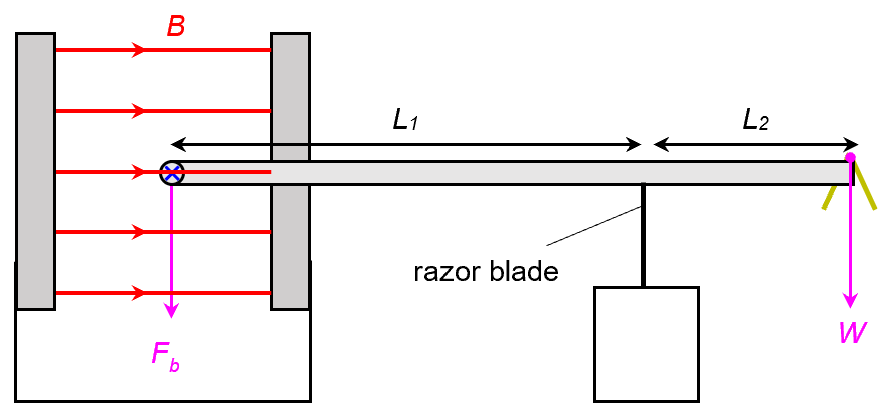
\includegraphics[scale=0.7]{media/Current Balance - Side View.png}
    \caption{The side view of the current balance.\protect\footnotemark[3]}
\end{figure}

The magnitude of $B$ can then be calculated by equation the anti-clockwise moment caused by the magnetic force $F = BIL$, and the clockwise moment caused by the weight $W$ about the razor blade pivot: \[\bp{BIL} L_1 = W L_2 \implies B = \frac{W}{IL} \frac{L_2}{L_1}.\]

\subsection{Moving Charge}

\begin{proposition}
    A charge $Q$ moving at velocity $v$ at an angle $\t$ to a uniform magnetic field of flux density $B$ will experience a force $F$ given by \[F = BQv\sin\t.\]
\end{proposition}
\begin{proof}
    Observe that \[IL = \bp{\frac{Q}{t}} L = Q \bp{\frac{L}{t}} = Qv,\] so \[F = BIL\sin\t = BQv\sin\t.\]
\end{proof}

\begin{proposition}
    If a charged particle enters a uniform magnetic field at a right-angle to the flux, its path in the field will be circular with radius \[r = \frac{mv}{QB},\] where $m$ is the mass of the particle, $v$ its velocity and $Q$ its charge.\protect\footnotemark
\end{proposition}
\begin{proof}
    By Fleming's left-hand rule, the velocity $v$ of the particle is perpendicular to the magnetic field $B$, thus the magnetic force provides the centripetal force for the particle to move in a circle. Equating the two, we see that \[BQv\sin90\deg = \frac{mv^2}{r} \implies r = \frac{mv}{QB}.\]
\end{proof}
\footnote{A similar result holds when the particle enters the field at an angle. In this case, however, the particle will move in a helical path.}

\begin{corollary}
    The period of revolution of the particle is independent of its speed.
\end{corollary}
\begin{proof}
    We have \[T = \frac{2\pi r}{v} = \frac{2\pi\bp{\frac{mv}{QB}}}{v} = \frac{2\pi m}{Bq},\] which is independent of $v$.
\end{proof}

\subsubsection{Velocity Selector}

Uniform magnetic and electric fields that are perpendicular to each other can be used to select charged particles of a particular speed. This arrangement produces forces opposite in directions acting on a beam of charged particles passing through the fields.

\begin{figure}[H]
    \centering
    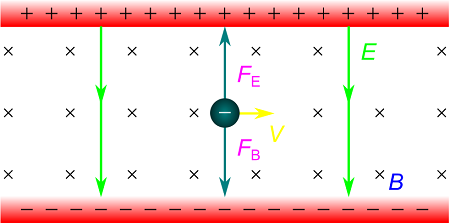
\includegraphics[scale=0.7]{media/Velocity Selector.png}
    \caption{An example of a velocity selector. Here, the magnetic field lines are into the page.}
\end{figure}

A particle of charge $Q$ and velocity $v$ will remain on a straight path if the magnitudes of the electric and magnetic forces are equal. The velocity at which this is achieved can be derived as follows: \[F_E = F_B \implies QE = QBv \implies v = \frac{E}{B}.\]

By changing the ratio of $E$ to $B$, charged particles of a certain selected speed may be collected from their undeflected path (hence the name velocity selection).